\subsection{问题2}
\subsubsection{模型建立}
本题需要设计以下参数:塔位置坐标 \((x_{R}, y_{R})\),定日镜镜面宽度 \(a\),镜面高度 \(b\),安装高度 \(d\),定日镜数目 \(N\)以及定日镜位置。

因为在一天之内,太阳方位角的变化是关于正午对称性变化,如下图所示
\begin{figure}[H]
\centering
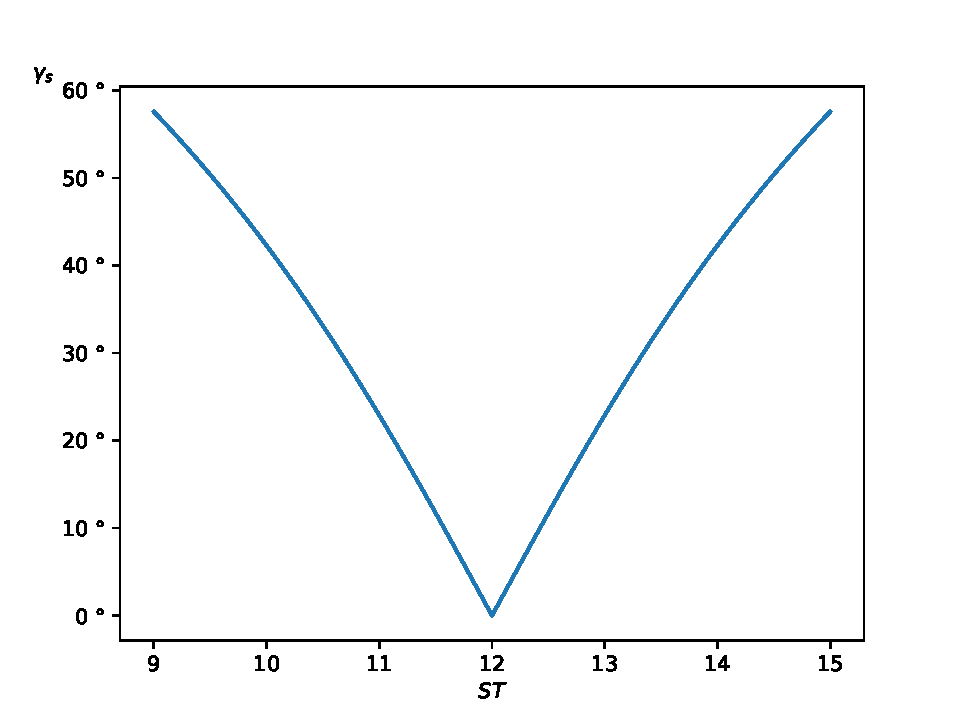
\includegraphics[scale = 0.4]{gammas.pdf}
\caption{\kaishu 太阳方位角 \(\gamma_{s}\)一天内关于时间的变化规律}
\end{figure}
于是能够确定中心塔一定位于定日镜镜场坐标系的 \(y\) 轴上,也即 \(x _{R} = 0\)。

又因为太阳入射方向沿 \(y\) 轴方向的分量总是正的,根据图~(\ref{north_south})和图~(\ref{rainbow})的分析结果可知,位于中心塔北边的定日镜光学效率会更高,于是为了使得位于中心塔北边的定日镜数目更多,中心塔应该位于定日镜镜场的南部,也即,\(y _{R} \in [-350 , 0]\)。

对于定日镜场的布局。本文采用均匀布局,以中心塔为圆心,在一定半径的圆周上等距地排列定日镜,并且相邻定日镜圈上之间的半径之差\(\Delta r\)相等,且据题目要求,同一圈上的相邻定日镜中心的距离设定为\(a +5\) m,定日镜距离中心塔的距离大于 \(100\) m。如下图所示,只保留位于镜场区域内的定日镜
\begin{figure}[H]
\centering
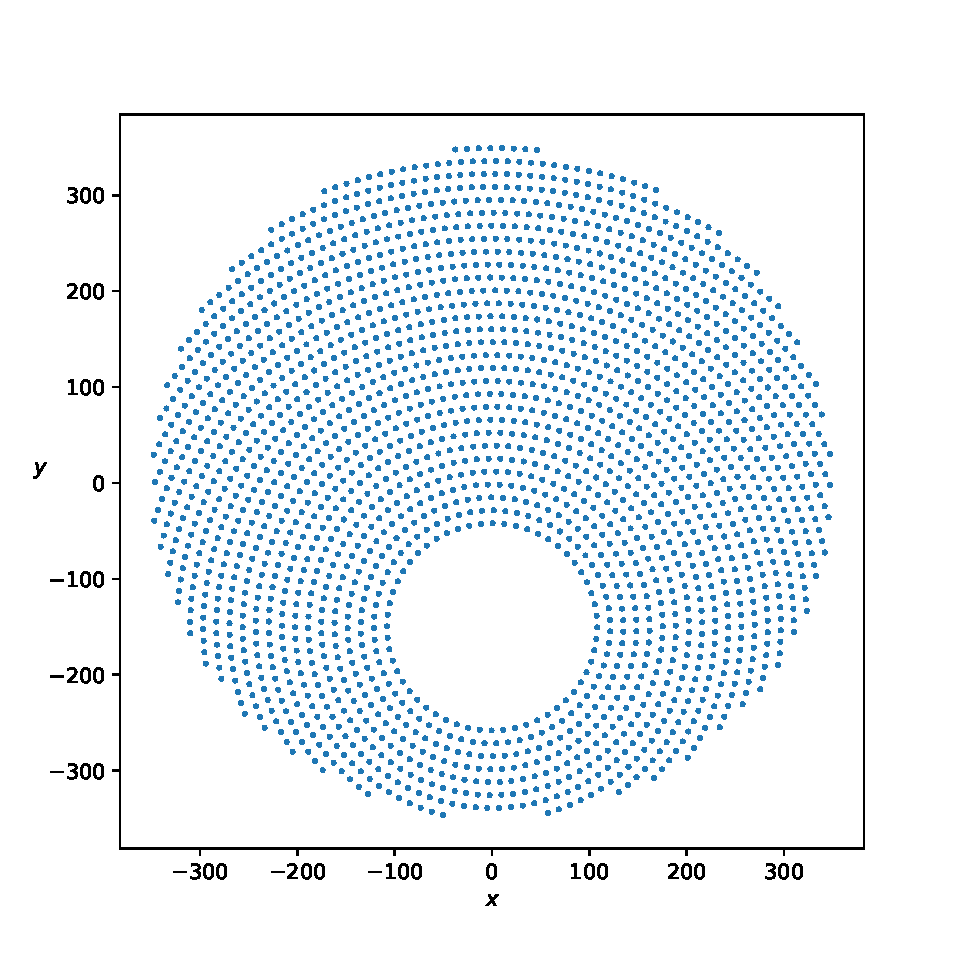
\includegraphics[scale = 0.5]{arange_2.pdf}
\caption{\kaishu 镜场均匀布局示意图}
\end{figure}
因此定日镜镜场的布局就可以用一个参数 \(\Delta r\)来描述,
同时,该参数也确定了定日镜数目 \(N\)。

根据题目信息,定日镜镜场的额定年平均输出热功率 \(P_{\mathrm{out}}\)为 \(60 \, \mathrm{MW}\),而优化目标为单位镜面面积年平均输出热功率最大,也即 \(\max \bar P_{\mathrm{out}}\),则问题可以转化为在额定功率下定日镜镜场的总镜面面积 \(S\)最小。

综上优化目标函数为
\begin{equation}
\min S = ab N
\end{equation}
决策变量为
\begin{equation}
\{ y_{R} , a , b , d, \Delta r \}
\end{equation}
约束条件为
\begin{equation}
s.t.
\begin{cases}
N = {\it getNumHelio} (y_{R} , a , \Delta r)\\
P_{\mathrm{out}} = 60 \,\mathrm{MW}\\
2 \le d \le 6\\
2 \le b \le a \le 8\\
\frac{b}{2} \sin (\max \varphi_{\text{水平转角}}) \le d
\end{cases}
\end{equation}

\subsubsection{模型求解}
% require GA.parent
\paragraph{使用遗传算法解决多决策变量的单目标优化问题}
遗传算法是借鉴生物界的进化规律演化而来的随机搜索方法,它可以在给定的复杂多维函数空间中进行搜索,以寻找函数的全局最优解或局部最优解。
可以分为以下步骤
\begin{itemize}
\item STEP A 生成染色体
本文将问题中所需要确定的吸收塔纵坐标\(y_{R}\),定日镜镜面宽度\(a\),定日镜镜面高度\(b\),定日镜安装高度\(h\),定日镜场排布半径间隔\(\Delta r\)在十进制内用基因表示每一位,并构成子染色体串,并把这些字串连接形成“染色体”。
\item 
STEP B    初始化种群
通过随机生成基因序列确定十进制编码之后,需要检验每个子染色体对应的十进制数是否在给定的上下限区间内,即\(y_{R} \in [-350 ,0]\),镜面边长\(a, b\)在2m到8m之间,\(d\)在2m到6m之间,\(\Delta r \in [10, 20]\)。当这一组基因序列满足以上要求,那么它将被收录到初始种群中,否则生成一组新的基因序列重复上述判断,直到达到最大种群规模数量max\_num时停止收录。
\item 
Step C   确定适应度函数
根据题意,为求单位镜面面积输出热功率最大,需要令镜面总面积最小,即
即刻画了适应度函数 \(\min \mathrm{Fitness}(x) = S = a  b  N\)
\item 
STEP D   转轮盘赌法确定优秀个体
在优秀筛选的过程中采用的是转轮盘赌法。其理论根据是:染色体的适应度越高,则它具有更大的概率被遗传到新一代种群中。
	
在这个轮盘上,有着从0到1的不均匀刻度,其中每两个刻度间的分度值由适应度函数来确定,轮盘最终停在某个刻度中,该刻度对应的染色体就遗传给后代种群。因此当计算出的总面积值越小时,刻度的分度值就越大,在轮盘上就越容易被选中,即被遗传的概率也越大。即在这种方法中,每一组基因序列被遗传的概率与其适应度函数的值成正比。
	
某染色体\(i\)对应的概率的计算(即\(i\)所对应的分度值):

\begin{equation}
P_{i} = \frac{{\it Fitness}(i)}{\sum_{k=1} ^{\text{max\_num}} {\it Fitness} (k)}
\end{equation}
	
染色体\(i\)的转轮盘赌累加概率的计算(染色体\(i\)的刻度值):

\begin{equation}
{\it sum P} = \sum_{k=1} ^{i} {\it Fitness} (k)
\end{equation}

在轮盘设计好之后,总共转动轮盘max\_num次,筛选出优秀个体。通过以下方式进行模拟:

生成(0,1]之间的随机数rand,在设计好的轮盘中找到大于rand的最小刻度,该刻度的值就是生成的新的个体,将其加入到新的后代种群中,
在获得规模为max\_num的新种群后,将该种群作为初始种群进行迭代,当迭代次数达到最大值之后,停止算法,返回该种群中的最优值。
\end{itemize}

	为了充分模拟生物学中染色体与基因的遗传规律,增加算法的局部搜索能力,在遗传的过程中,本文将考虑对染色体进行交叉和变异操作。
\begin{enumerate}
\item 
Crossover:
对于两个优秀染色体,进行交叉:即生成[0,4]内的随机数,当随机数为0时,交换这两个解染色体的\(y_{R}\)部分;当随机数为1时,交换这两个解染色体的a部分,以此类推。
\item 
Variation:
对于一个染色体的十进制序列,考虑到突变是具有随机性的,在序列的随机位置将其随机更换为另一个十进制数。
\end{enumerate}

\paragraph{参数设置}
遗传算法自身拥有4个决策变量,即最大种群规模max\_num,变异概率
Prob\_mut,交叉概率crossoverfraction,最大迭代次数max\_iter。本文中最大种群规模设为100,种群规模足够大,确保找到最优解的基础概率;变异概率为0.01,符合变异的自然规律;交叉概率为默认值0.8,让种群中优秀的基因充分交流,促进种群进化;最大迭代次数设为1000,在运行足够久的遗传之后,结果会向着更优解收敛。

最后得出结果如下

\footnote{根据研究表明,12个典型日中春分日的平均DNI值更接近于年均DNI值,为了保障合理性并且降低求解难度,现选择春分日 10 点30分作为镜场的设计点。}
% cite require
% TODO rearange require
%
\begin{table}[H]
\centering
\input tab_2_1.tex
\caption{\kaishu 问题2每月21日平均光学效率及输出功率}
\end{table}
%
\begin{table}[H]
\centering
\input tab_2_2.tex
\caption{\kaishu 问题2年平均光学效率及输出功率表}
\end{table}
%
\begin{table}[H]
\centering
\input tab_2_3.tex
\caption{\kaishu 问题2设计参数表}
\end{table}
%

\subsubsection{模型分析}
本文发现在问题2的模型求解过程之中,决策变量会收敛到两类不同的取值。对于第一种,吸收塔的坐标位于最南端,没有定日镜位于吸收塔的正南部;对于第二种,仍有定日镜位于吸收塔的正南端,如下图所示
\begin{figure}[H]
\centering
\begin{subfigure}[b]{0.4\textwidth}
\centering
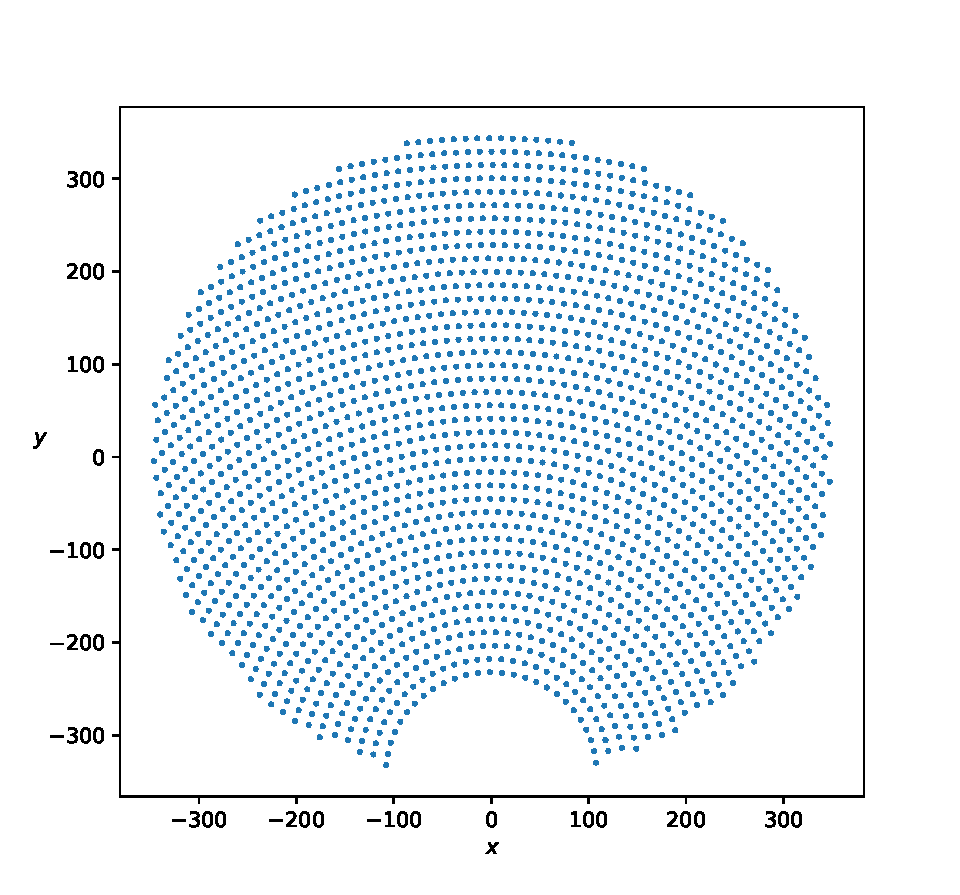
\includegraphics[scale = 0.3]{north_field.pdf}
\caption{\kaishu {\rm north field} 布局}
\end{subfigure}
\begin{subfigure}[b]{0.4\textwidth}
\centering
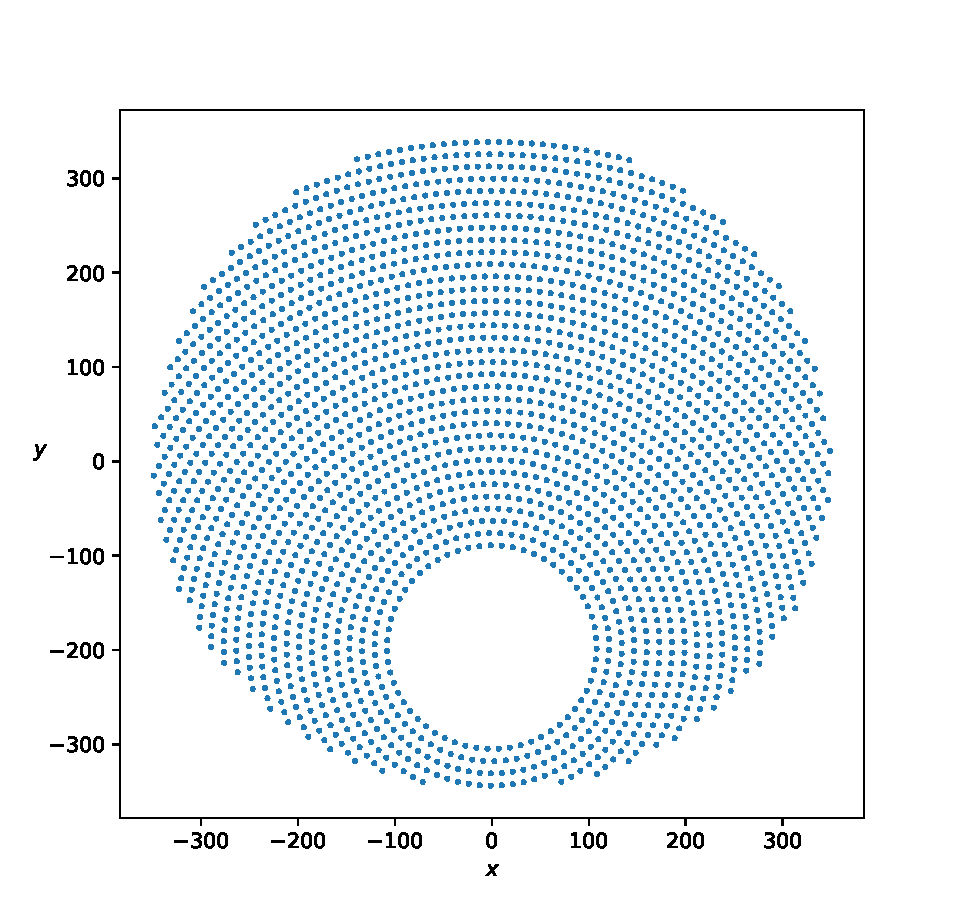
\includegraphics[scale = 0.3]{circular.pdf}
\caption{\kaishu {\rm circular} 布局}
\end{subfigure}
\caption{两种布局的示意图}
\end{figure}
查阅资料可知,上述两种布局分别称为 north field 和 circular 布局 \cite{zhangML},north field 布局并不常用于圆形镜场的布局之中,故本文采用 circular 布局。
下图是将各个指标随月份变化的现对该结果进行分析。
%
\begin{figure}[H]
\centering
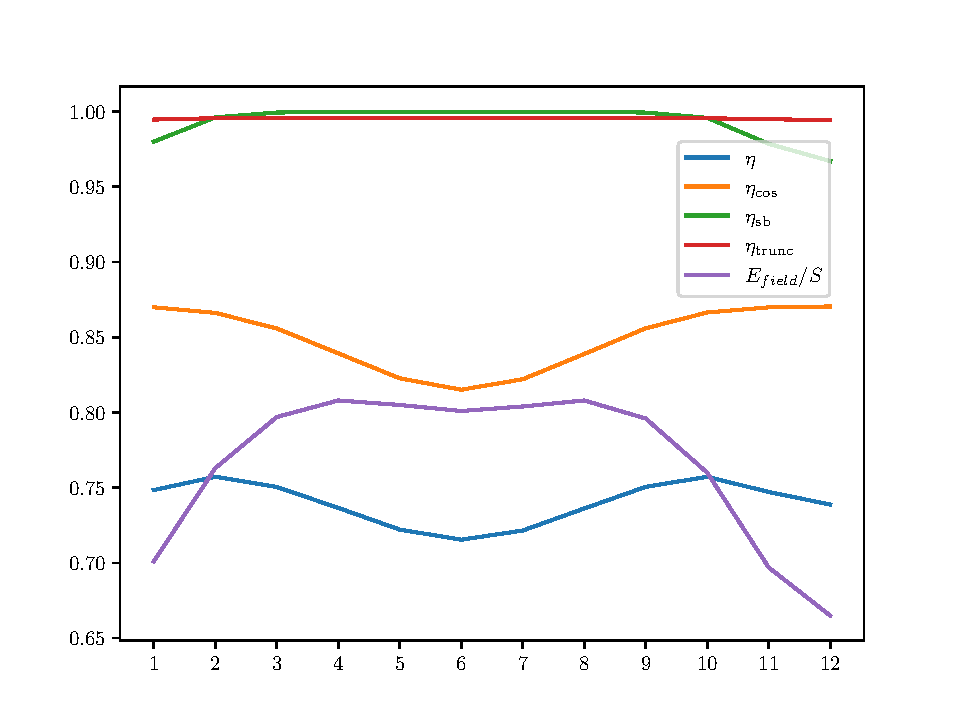
\includegraphics[scale=0.5]{zhexiantu2.pdf}
\caption{\kaishu 问题2设计之中各个指标随月份变化折线图}\label{fig:zhexiantu2}
\end{figure}
%
首先,在问题二的设计布局下,定日镜场的截断效率保持在0.996,左右,周围仅有微小扰动;阴影遮挡效率仅在冬季(即11,12,1月份)出现小幅度的下降,其他月份均接近1,与实际情况相符;

对于余弦效率为什么在冬至取得最大,从冬至到夏至的过程中不断减小,本文给出的合理性分析是:由于定日镜场在南北方向上呈不对称分布,在北面的定日镜数目远大于南面的定日镜。根据图(\ref{summer_winter})可以看出,在夏季由于正午太阳高度角更高,导致其入射光与反射光所成的角度越大,这样造成的余弦损失就越大。
%
\begin{figure}[H]
\centering
\input summer_winter.tex
\caption{\kaishu 冬季夏季的余弦效率示意图}\label{summer_winter}
\end{figure}
%
% 在上述两个因素,即\(\eta _{\mathrm{s b}}\)和\(\eta _{\cos}\)的同时作用下,
而定日镜的光学效率 \(\eta\),受余弦效率影响较大 \cite{zhangML},于是
\(\eta\)和单位面积年平均输出热功率\(E_{\mathrm{field}}/S\)就呈现如图的关于夏至对称的变化折线形状。

下图是春分15:00时定日镜场可视化的结果。由图可以看出,在模拟结果之中位于东北侧的定日镜的光学效率显著高于西南侧的,这是因为春分日下午15:00时,太阳光入射方向为由西南到东北;位于内圈有一定日镜的光学效率特别低,这是因为该定日镜被吸收塔的阴影遮挡了大部分镜面。由上分析可知该结果和实际相符。
%
\begin{figure}[H]
\centering
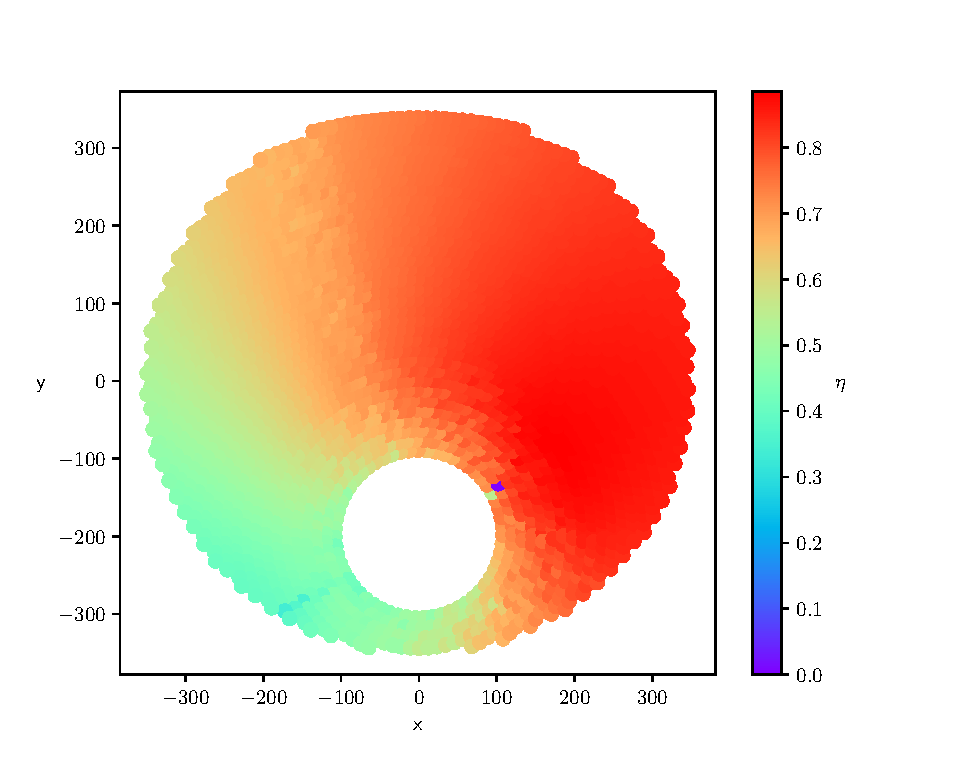
\includegraphics[scale = 0.7]{rainbow2.pdf}
\caption{\kaishu 春分{\rm 15:00}时分镜场内各个定日镜光学效率可视化结果}\label{rainbow2}
\end{figure}
